\newcommand\sHeigh{.75cm}
\newcommand\sWidth{1cm}
\newcommand\cHeigh{.75cm}


\usetikzlibrary{shapes.geometric, arrows}
\tikzstyle{block} = [rectangle, minimum height=\sHeigh,text centered, draw=black,font=\footnotesize]
\tikzstyle{sp} = [rectangle, minimum width=\sWidth, minimum height=\sHeigh,text width=\sWidth,text centered,font=\footnotesize]
\tikzstyle{sum} = [circle,minimum width=\cHeigh,font=\footnotesize,draw=black]
\tikzstyle{arrow} = [thick,->,>=stealth]

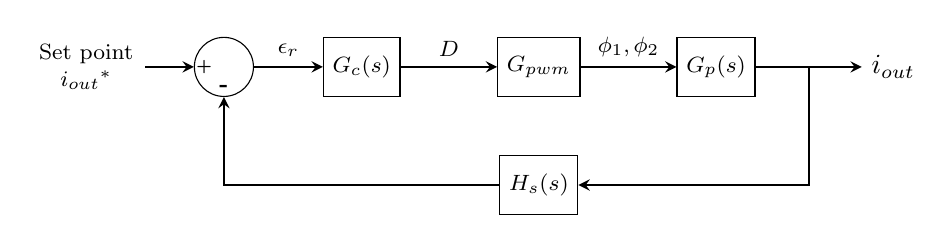
\begin{tikzpicture} [node distance = 2.25cm]
\node (sp) [sp,text width=1.25cm] {Set point\\ ${i_{out}}^*$};
\node (error) [sum,right of =sp, xshift=-0.5cm] {};
\node (comp) [block, right of = error, xshift=-0.5cm] {$G_c(s)$};
\node (pwm) [block, right of = comp] {$G_{pwm}$ };
\node (H-SCC) [block,right of = pwm] { $G_p (s)$};
\node (sens) [block,below of = pwm,yshift=+0.75cm] {$H_s(s)$};
\node (out) [right of = H-SCC] {$i_{out}$};

\draw [arrow] (sp) -- (error)node[font=\tiny,xshift=-0.25cm]{\textbf{+}};
\draw [arrow] (error) --node[font=\footnotesize,anchor=south]{$\epsilon _r$} (comp);
\draw [arrow] (comp) --node[font=\footnotesize,anchor=south]{$D$} (pwm);
\draw [arrow] (pwm)--node[font=\footnotesize,anchor=south]{$\phi_1,\phi_2$} (H-SCC);
\draw [arrow] (H-SCC) --node(x_out)[yshift=0.12cm]{} (out);
\draw [arrow] (x_out) |- (sens);
\draw [arrow] (sens) -| (error)node[font=\footnotesize,yshift=-0.25cm]{\textbf{-}};






\end{tikzpicture}
